\documentclass[a4paper,12pt]{article}

%%% Работа с русским языком

%%% Дополнительная работа с математикой
\usepackage{amsfonts,amssymb,amsthm,mathtools} % AMS
\usepackage{amsmath}
\usepackage{icomma} % "Умная" запятая: $0,2$ --- число, $0, 2$ --- перечисление

%% Номера формул
%\mathtoolsset{showonlyrefs=true} % Показывать номера только у тех формул, на которые есть \eqref{} в тексте.

%\usepackage{hyperref}
%\hypersetup{
%    colorlinks=true,
%    linkcolor=blue,
%    filecolor=magenta,      
%    urlcolor=cyan,
%}

\usepackage{float}


%% Шрифты
\usepackage{euscript}	 % Шрифт Евклид
\usepackage{mathrsfs} % Красивый матшрифт

%%% Работа с картинками
\usepackage{graphicx}  % Для вставки рисунков
%\graphicspath{{images/}{images2/}}  % папки с картинками
\setlength\fboxsep{3pt} % Отступ рамки \fbox{} от рисунка
\setlength\fboxrule{1pt} % Толщина линий рамки \fbox{}
\usepackage{wrapfig} % Обтекание рисунков и таблиц текстом
\usepackage{caption}
\usepackage{subcaption}
\captionsetup{labelsep=period} %. вместо : в рис

\title{Simulations of the Nowak-May game in three spatial dimensions}
\author{Moskalenko Roman \\ HSE
\and Burovski Evgeni}
\date{October \\ 2020}

\begin{document}

\maketitle

\section{Introduction}

We study the evolutionary spatially distributed game of Nowak and May \cite{nowak and may 1}, \cite{nowak and may 2}. Based on the Prisoner’s Dilemma this model defines evolution of cooperation in group of agents, which are arranged in a pattern. In the original work pattern was a square lattice. This two-dimensional game has a variety of different regimes. But what happens when we change the pattern from two-dimensional square lattice to three-dimensional cubic lattice. In this paper we look at the dynamics of the game on cubic lattice.


\section{Game description}

The game is based on the Prisoner’s Dilemma. In this variation of the dilemma we have two agents follow one of two strategies cooperate or defect. Agents play with each other and get points depending on what strategy both of them use according to this table. Nowak and May's original game uses a square grid on which agents are located. Each step of the game agents play with their neighbors and get points according to the table \ref{fig:score table}. Then after all points are scored agents change their strategy to the strategy of the neighbor with the best score.

\begin{figure}[h]
	\centering
	\begin{subfigure}[b]{0.4\textwidth}
		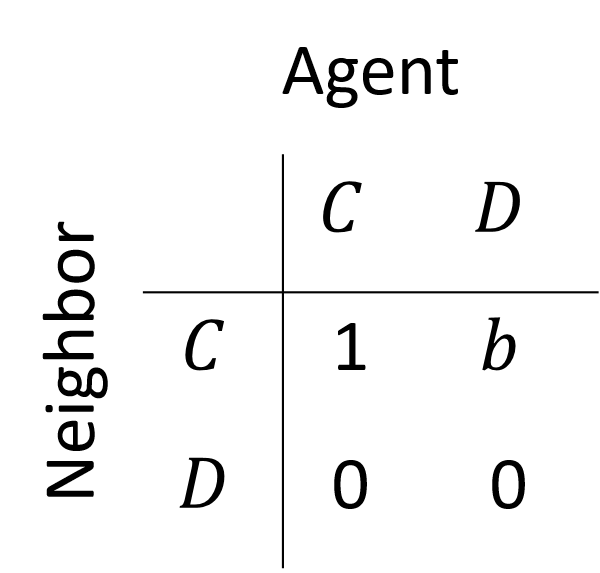
\includegraphics[width = \textwidth]{Game_score_table.png}
		\caption{Score table}	
		\label{fig:score table}	
	\end{subfigure}
	\begin{subfigure}[b]{0.4\textwidth}
		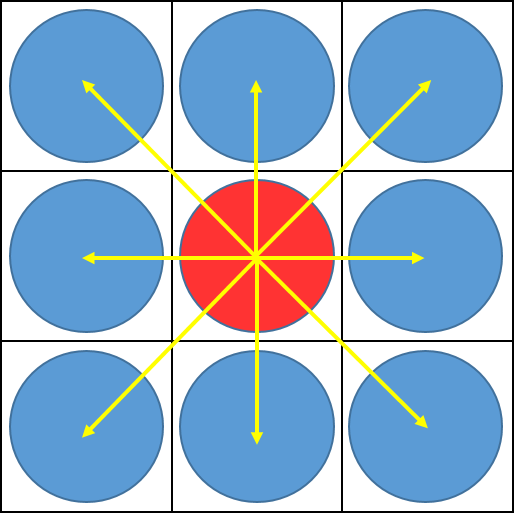
\includegraphics[width = \textwidth]{Games_with_neighbors_pic.png}
		\caption{Square lattice neighbors}
	\end{subfigure}
	\caption{}
\end{figure}


Apart from the initial state, the game is completely determined by the parameter $b$, then how this parameter affects the game and is of greatest interest to us.

On cubic lattice, the game goes according to the same rules. The major change is that every agent now has 27 neighbors (including themselves) instead of 9. It is important because not all possible values of parameter $b$ correspond to unique regime of the game. There are transition points, for all values between them the game is identical. These points are rational fractions with the numerator and denominator have values from one to number of neighbors. Therefor number of possible unique regimes increases significantly.

\section{Current results}

We have measured some key parameters of the game: concentration of cooperators \ref{fig:Fc}, strategy change time \ref{fig:change time} and persistence \ref{fig:persistence}.

Concentration of cooperators is the number of cooperators divided by the number of all agents. Strategy change time is mean time for agents to change strategy. Persistence is fraction of agents who have not changed their strategy after stabilization of the field.


These measurements  largely describe the behavior of the game. For example we can see sharp decrease of the concentration of cooperators at points like $b = \frac{27}{n}, n\in\{1, 2, \ldots, 27\} $. It happens because when $b > \frac{27}{n}$ isolated groups of $n$ or more defectors will grow and their neighbors will become defectors. There are also some things that we have not currently explain. Like why does the concentration of cooperators sometimes increases with greater $b$ values. 

\begin{figure}[H]
	\centering
	
	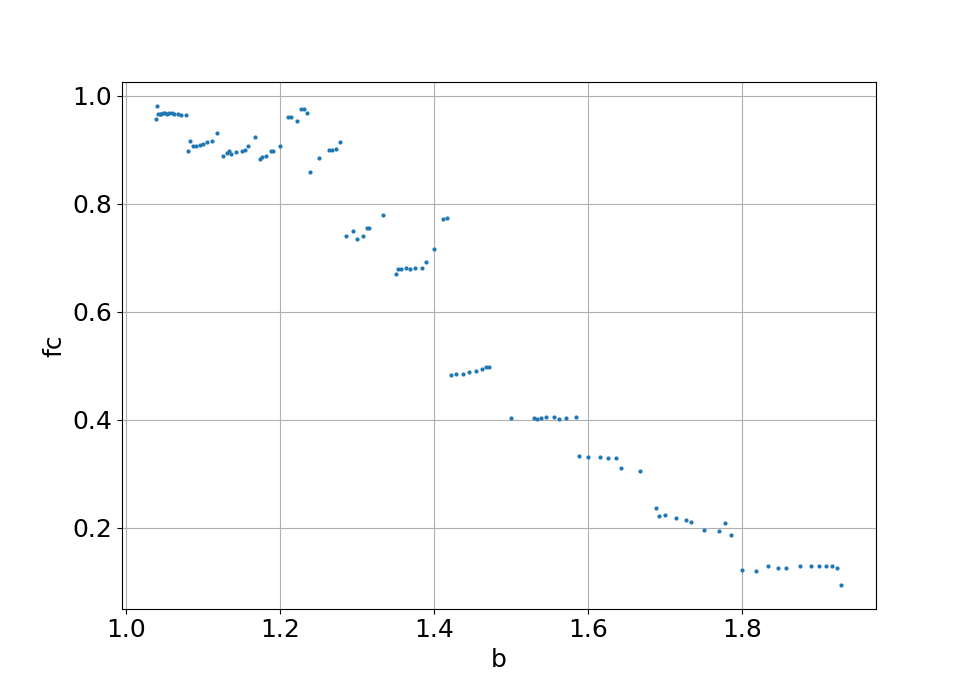
\includegraphics[width = \textwidth]{C_0.9_graph.png}
	\caption{Mean concentration of cooperators, each value is the average of ten independent fields, 100 measurements were taken on each field every 100 evolution steps	}
	\label{fig:Fc}

\end{figure}



But the concentration does not describes how exactly does agents change the strategy. For this we look at the strategy change time and persistence. Persistence is fraction of agents who does not change their strategy over some period of time. 

\begin{figure}[H]
	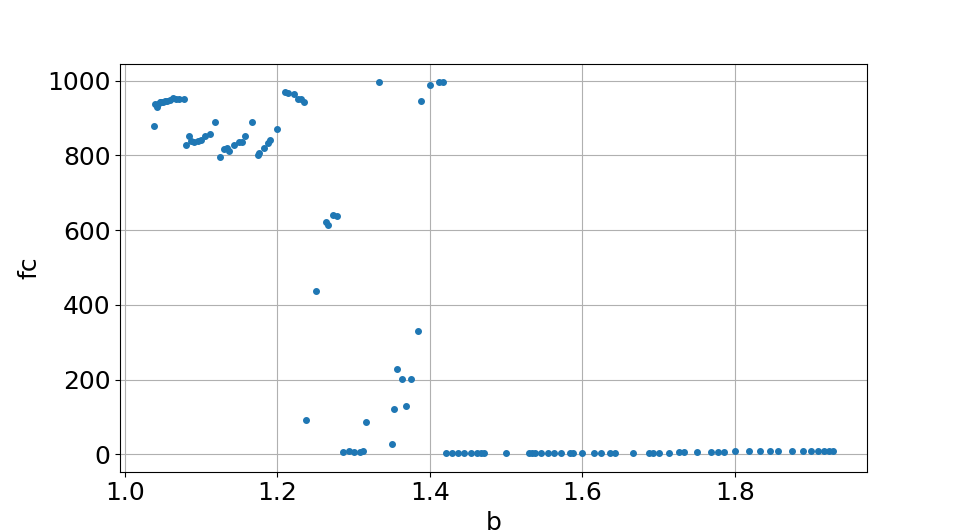
\includegraphics[width = \textwidth]{Change_time.png}
	\caption{Mean strategy change time}
	\label{fig:change time}
\end{figure}

\begin{figure}[h]
	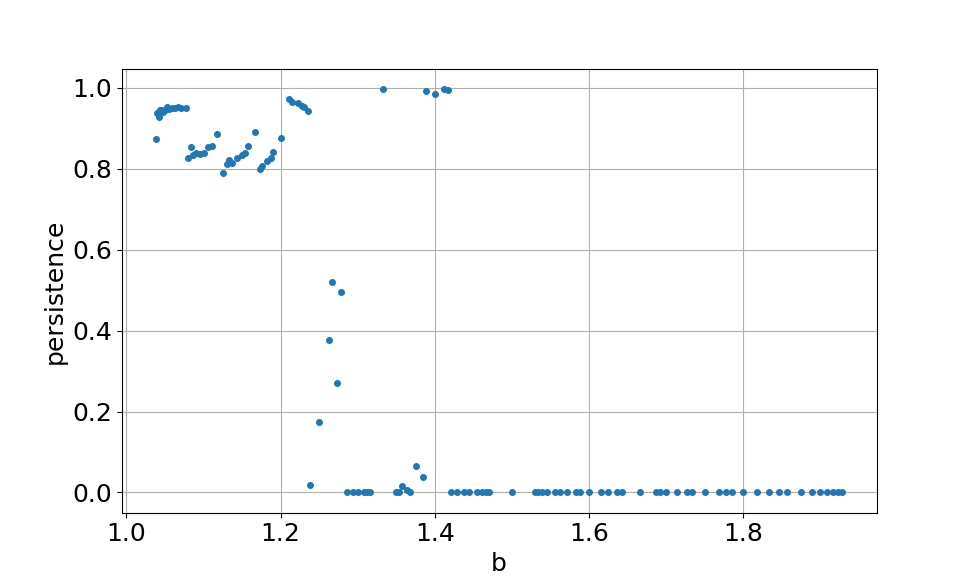
\includegraphics[width = \textwidth]{Persistence.png}
	\caption{Persistence}
	\label{fig:persistence}
\end{figure}

As we can see from graphs \ref{fig:change time} and \ref{fig:persistence} strategy change time and persistence are strongly related. For $b\in(1, 1.24)$ persistence and change time almost proportional to each other and even to concentration of cooperators. It is because at these low values of $b$ defectors are separated in small isolated groups and agents around thous groups are constantly changing their strategy back and forth. Thus number of agents who change strategy is proportional to the number of defectors. than around $b \approx 1.3$ there are some chaotic regimes where most of the agents very frequently changing their strategy. Also there are some anomalies around $b = 1.4$. For some reason almost all agents stop changing their strategy at those points but not all of them. And not only agents stop changing their strategy, but concentration of cooperators also increases. 

\subsection{The impact of the field}
In addition to the above measurements, we checked the results of the game on fields of various sizes and with different initial distributions of strategies.

Most all of the previous measurements were taken on a $60\times60\times60$ field because smaller fields are more dependent on the initial situation on the field. And natural question is what happens on larger fields.


\begin{figure}[h]
	\centering
	
	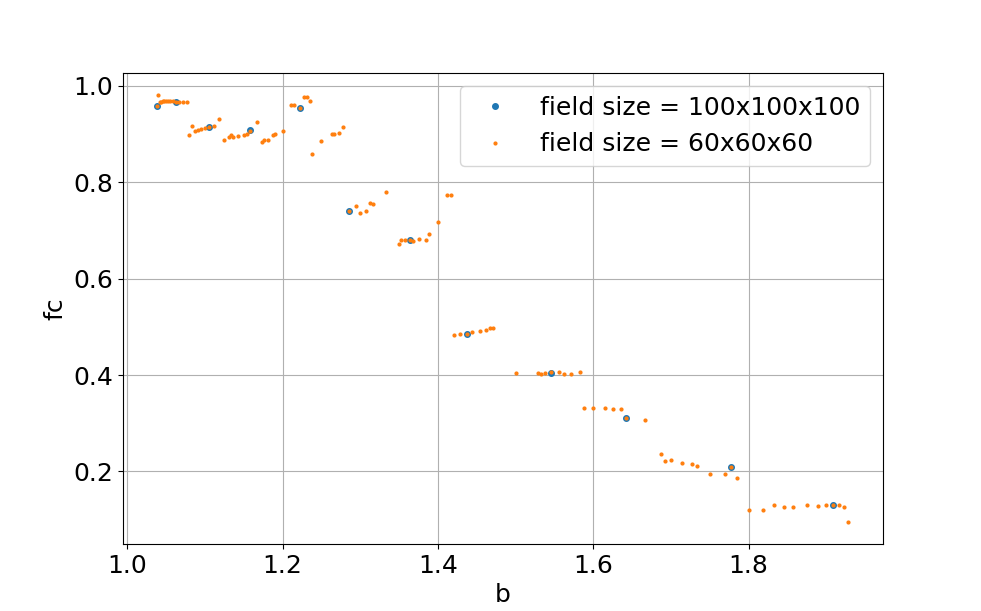
\includegraphics[width = \textwidth]{Fc_60_and_100.png}
	\caption{Mean concentration of cooperators on $60\times60\times60$ and $100\times100\times100$	}
	\label{fig:Fc100}

\end{figure}

As we can see on graph \ref{fig:Fc100} values on fields of both sizes are identical. So all big enough fields give us identical behavior of the game.

Initial strategies of agents obviously affect the game. Even at the lowest values of $b$ there is a chance that all of the agents will become defectors and vice versa. To find out how exactly initial field affects the game we have measured concentration of cooperators on fields with different initial concentration of cooperators.

\begin{figure}[h]
	\centering
	\begin{subfigure}[b]{0.48\textwidth}
		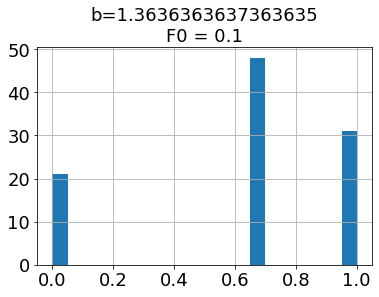
\includegraphics[width = \textwidth]{b1,3_Fc0,1_hist.png}
		\caption{$Fc0 \approx 0.1$}
	\end{subfigure}
	\begin{subfigure}[b]{0.48\textwidth}
		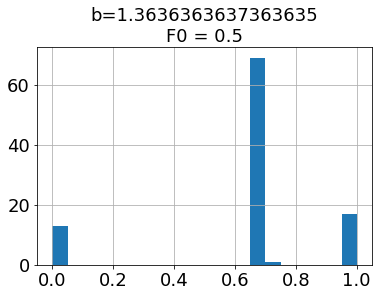
\includegraphics[width = \textwidth]{b1,3_Fc0,5_hist.png}
		\caption{$Fc0 \approx 0.5$}
	\end{subfigure}
	\begin{subfigure}[b]{0.48\textwidth}
		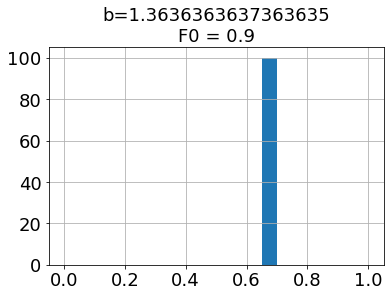
\includegraphics[width = \textwidth]{b1,3_Fc0,9_hist.png}
		\caption{$Fc0 \approx 0.9$}
	\end{subfigure}
	
	\caption{Histograms of distribution of 100 independent fields by concentration of cooperators with corresponding initial concentrations, $b\approx 1.3637$}
	\label{fig:Fc0 hist}
\end{figure}

It appears that the lower the initial concentration the higher the chances that all of the agents will come to the same strategy. For example on histograms \ref{fig:Fc0 hist} we can see that with initial concentration 0.1 and 0.5 a big portion of fields falls to values of 1 and 0. But all the other fields come to the same value  as the fields with initial concentration of 0.9. So apart from the fields that fall to the extreme values concentration of cooperators does not depend on initial strategies of agents.


\begin{thebibliography}{9}

\bibitem{github}
Github repository: https://github.com/MoskalenkoRomanBorisovich/Spatial-Distribution-Evolutionary-Game. 

\bibitem{nowak and may 1}
M.A. Nowak and R.M. May, Evolutionary games and spatial chaos, Nature 359, 826 (1992).

\bibitem{nowak and may 2}
M.A. Nowak, Evolutionary Dynamics: Exploring the equations of life, The Belknap Press, (2006).

\end{thebibliography}

\end{document}
